\documentclass[]{article}
\usepackage[utf8]{inputenc}
\usepackage{pdfpages}
\usepackage{amsmath}
\usepackage{amssymb}
\usepackage{graphicx}
\usepackage{geometry}
\usepackage{enumitem}
\usepackage{amsthm}

\usepackage{graphicx}
\usepackage{geometry}

\geometry{hmargin=2cm}

\title{Analyse}

\author{Isabelle Galagher et Pierre Gervais}

% Environnement type théorème
\newtheorem{mythm}{Théorème}
\newtheorem{myproposition}{Proposition}
\newtheorem{myproperty}{Propriété}
\newtheorem{mylemma}{Lemme}

% Environnement type texte
\theoremstyle{remark}
\newtheorem{myrem}{Remarque}
\newtheorem{myexer}{Exercice}
\newtheorem{myproof}{Preuve}
\newtheorem{myexmpl}{Exemple}

% Environnement de définition
\theoremstyle{definition}
\newtheorem{mydef}{Définition}

\setlist[itemize]{label=-}

% Carré de fin de preuve
\newcommand{\cqfd}{
	\hfill$\square$
}

% Définition de fonction
\newcommand{\func}[5]{
#1 ~ : ~ \left\{ \begin{array}{lcl}
	#2 & \longrightarrow & #3 \\
	#4 & \longmapsto & #5
\end{array}
\right.
}

\begin{document}

\maketitle

\tableofcontents

\part{Topologie des espaces vectoriels normés}

\section{Espaces vectoriels normés : premières définitions}

\subsection{Distances et normes}

\begin{mydef}
	Étant donné un ensemble $E$, une \textit{distance sur $E$} est une application $d~: ~ E \times E \longrightarrow \mathbb{R}$ vérifiant les propriétés suivantes :
	\begin{enumerate}
		\item $d$ est \textit{définie positive} : $d(x,y) \geqslant 0$ et $d(x,y) = 0 \Leftrightarrow x=y$
		\item $d$ est symétrique : $d(x,y)=d(y,x)$
		\item $d$ vérifie l'\textit{inégalité triangulaire} : $\forall z \in E, ~ d(x,y) \leqslant d(x,z) + d(z, y)$
	\end{enumerate}
\end{mydef}

\begin{myexmpl}
	\leavevmode
	\begin{itemize}
		\item $E=\mathbb{R}$ et $d(x, y) = |x-y|$
		\item $E=\mathbb{R}^2$ et $d\left(\binom{a}{b},\binom{c}{d}\right)=\sqrt{(a-c)^2+(b-d)^2}$
	\end{itemize}
\end{myexmpl}

\begin{myrem}
	Par l'inégalité triangulaire, on déduit
	\begin{itemize}
		\item $d(x,z) \geqslant d(x, y) - d(y, z)$
		\item $d(x, z) \geqslant d(z, y) - d(x, y)$
	\end{itemize}
	d'où $|d(x, y) - d(z, y)| \leqslant d(x, z)$
\end{myrem}

\begin{mydef}
	Soit $E$ un $\mathbb{K}$-espace vectoriel, une \textit{norme} sur $E$ est une application notée $N$ ou $\|\cdot\|$ telle que
	\begin{enumerate}
		\item $(x, y) \longmapsto \|x - y\|$ est une distance
		\item $\forall \lambda \in \mathbb{R}, ~ \forall u \in E, ~ \|\lambda u\| = |\lambda|\|u\|$ (\textit{homogénéité})
	\end{enumerate}
\end{mydef}

\begin{myproposition}
	Une fonction $\|\cdot\| ~ : ~ E \longrightarrow \mathbb{R}$ est une norme si et seulement si :
	\begin{enumerate}
		\item elle est homogène
		\item elle est définie
		\item elle vérifie l'inégalité triangulaire
	\end{enumerate}
\end{myproposition}

\begin{myproof}
	\leavevmode
	
	{\boldmath $\Longrightarrow$}
	
	Soit $\|\cdot\|$ une norme.
	\begin{enumerate}
		\item \checkmark
		\item $\|x\|=d(x, 0)$ où $d(x,y)=\|x-y\|$, donc $\|x\| \geqslant 0$ et $\|x\|=0 \Longleftrightarrow d(x, 0)=0 \Longleftrightarrow x=0$
		\item $\|x+y\| = d(x+y, 0) = d(x, -y)$, or $\forall x, y, z \in E, ~ d(x, z) \leqslant d(x, y) + d(y, z)$ donc $d(x, -y) \leqslant d(x, 0) + d(0, -y)$
		D'où $\|x+y\| \leqslant d(x, 0) + d(0, -y) \leqslant \|x\| + \|-y\| \leqslant \|x\| + \|y\|$
	\end{enumerate}
	
	{\boldmath $\Longleftarrow$}
	
	Soit $\| \cdot \|$ vérifiant les trois propriétés, alors soit $d(x, y)=\|x-y\|$ et montrons que d est une distance.
	
	\begin{enumerate}
		\item $d(x, y) \geqslant 0$ car $\|x-y\| \geqslant 0$ par (2).
		$d(x, y) = 0 \Longleftrightarrow \|x-y\| = 0 \Longleftrightarrow x = y$
		
		\item $d(x, y) = \|x-y\|=\|-(x-y)\| = \|y-x\|=d(y, x)$
		
		\item $d(x, y) = \|x-y\| = \|x-z + z - y\| \leqslant \|x-z\| +\|z-x\| \leqslant d(x, y) + d(z, y)$
 	\end{enumerate}
\end{myproof}

\begin{myexmpl}
	\leavevmode
	\begin{enumerate}
		\item Dans $\mathbb{R}^n$, on définit les normes $\displaystyle \|x\|_1= \sum_{k=1}^n |x_k|$, $\displaystyle \|x\|_2 =  \sqrt{\sum_{k=1}^n |x_k|^2}$, $\displaystyle \|x\|_p = \sqrt[p]{\sum_{k=1}^n |x_k|^p}$ et $\displaystyle \|x\|_\infty = \max_{k} \|x_k\|$
		\item Dans $\mathbb{R}^n$ muni d'un produit scalaire, $\|x\| = \sqrt{\langle x, x\rangle}$
		\item Soit $A$ un ensemble et $F$ une espace vectoriel normé, et $\mathcal{B}(A, F)$ les fonctions bornées de $A$ dans $F$, alors $\displaystyle \|f\|_\infty = \sup_{x \in A} \|f(x)\|$ est une norme.
		\item Sur $\mathcal{C}([0, 1], \mathbb{R})$, $\displaystyle \|f\|_1 = \int_{0}^{1}\left|f(x)\right|$, $\displaystyle \|f\|_2 = \sqrt{\int_{0}^{1}\left|f(x)\right|^2}$ et$\displaystyle \|f\|_\infty = \sup_{0 \leqslant x \leqslant 1}\left|f(x)\right|$
	\end{enumerate}
\end{myexmpl}

\begin{mydef}
	Deux normes $N_1$ et $N_2$ sont dites \textit{équivalentes} s'il existe des constantes positives $C_1$ et $C_2$ telles que $\forall x \in E, ~ C_1 N_2(x) \leqslant N_1(x) \leqslant C_2 N_2(x)$
\end{mydef}

\begin{myexmpl}
	Par exemple dans $\mathbb{R}^n$, les normes $\|\cdot\|_1$, $\|\cdot\|_2$ et $\|\cdot\|_\infty$ sont équivalentes. En effet $$\|x\|_1=|x_1|+|x_2| \leqslant 2 \|x\|_\infty$$ et $\|x_i| \geqslant \|x\|_\infty, ~ i=1, 2$
\end{myexmpl}

En dimension finie, toutes les normes sont équivalentes ! Cela n'est en revanche pas vraie en dimension infinie.

\begin{figure}[h!]
	\centering
	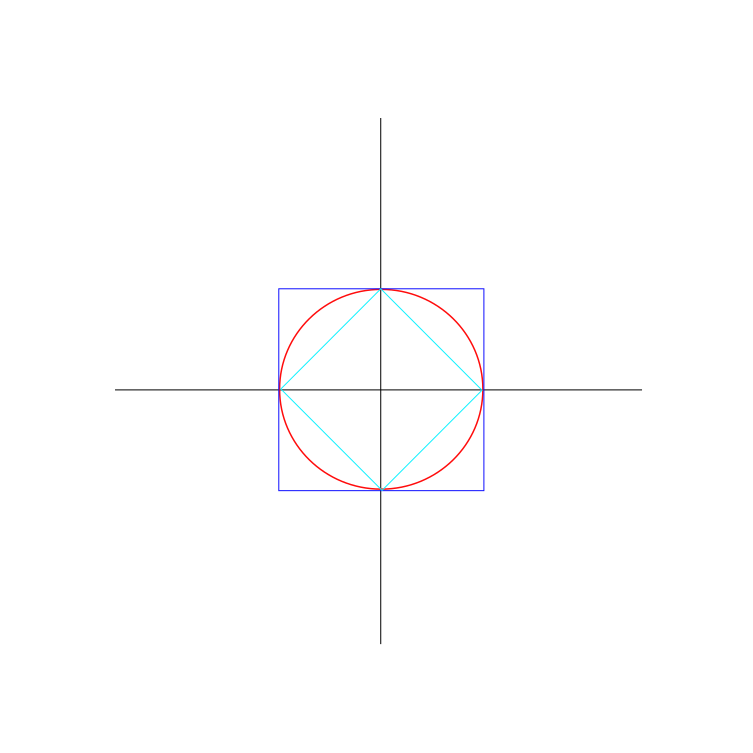
\includegraphics[width=350pt]{Schema1}
	\caption{Différentes boules unités}
	En bleu : $\mathcal{B}_\infty(0, 1)$
	
	En rouge : $\mathcal{B}_2(0, 1)$
	
	En turquoise : $\mathcal{B}_1(0, 1)$
\end{figure}

\subsection{Ouverts et fermés}

\begin{mydef}
	Soit $E$ un espace vectoriel normé, on appelle \textit{boule fermée} de centre $x$ et de rayon $r > 0$ l'ensemble $\overline{\mathcal{B}}(x, r) = \{u \in E ~|~ \|x-u\| \leqslant r\}$, et la \textit{boule ouverte} de centre $x$ et de rayon $r > 0$ l'ensemble $\mathcal{B}(x, r) = \{u \in E ~|~ \|x-u\| < r\}$.
\end{mydef}

\begin{mydef}
	Soit $X \subseteq E$
	\begin{enumerate}
		\item On dit que $U \subseteq X$ est un \textit{ouvert} de $X$ si $\forall x \in U, ~ \exists r > 0 ~ : ~ \mathcal{B}(x, r) \cap X \subseteq U$
		\item On dit que $F \subseteq X$ est un \textit{fermé} de $X$ si son complémentaire dans $X$ est un ouvert de $X$.
	\end{enumerate}
\end{mydef}

\begin{figure}[h!]
	\centering
	\includegraphics[width=200pt]{Ouverts_fermes}	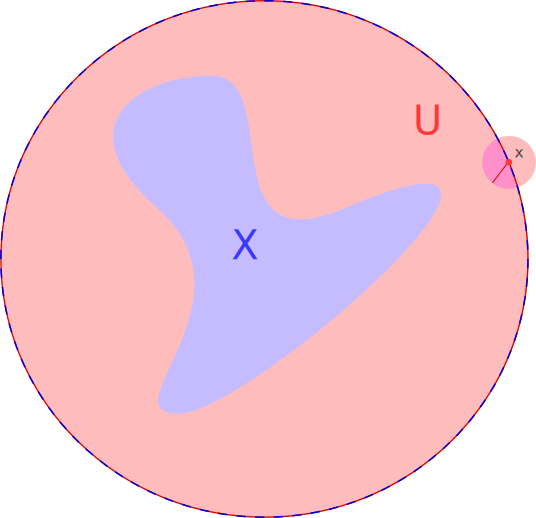
\includegraphics[width=200pt]{Ouverts_fermes2}
	\caption{Deux exemples d'ouverts}
\end{figure}

\begin{myrem}
	\leavevmode
	\begin{enumerate}
		\item Un ouvert dans $X$ n'est pas nécessairement ouvert dans $E$, comme montré dans le deuxième exemple de la figure ci-dessus.
		\item Un ouvert de $E$ sera appelé un \textbf{ouvert}, de même pour les fermés.
		
		\item Toute boule ouverte est un ouvert.
		
		\item Toute boule fermée est un fermé.
	\end{enumerate}
\end{myrem}

\newpage

\begin{myproof}
	On considère une boule ouverte $\mathcal{B}(x_0, r)$, montrons que c'est un ouvert.
	
	Soit $x \in \mathcal{B}(x_0, r)$, alors $\|x-x_0\| < r$. On cherche $r'$ tel que $\mathcal{B}(x, r') \subseteq \mathcal{B}(x_0, r)$ donc $r'$ doit vérifier $$\|x-y\| < r' \Longrightarrow \|x_0-y\| < r$$.
	
	Mais $\|x_0-y\| \leqslant \|x-y\| + \|x-x_0\| < \|x-y\| + r$.
	
	Soit $\delta = r - \|x-x_0\| > 0$, on pose alors $r'=\frac{\delta}{2} > 0$, alors $\|x_0-y\| \leqslant r' + \|x-x_0\| \leqslant r' + r - \delta < r$

	\cqfd
\end{myproof}

\begin{figure}[h!]
	\centering
	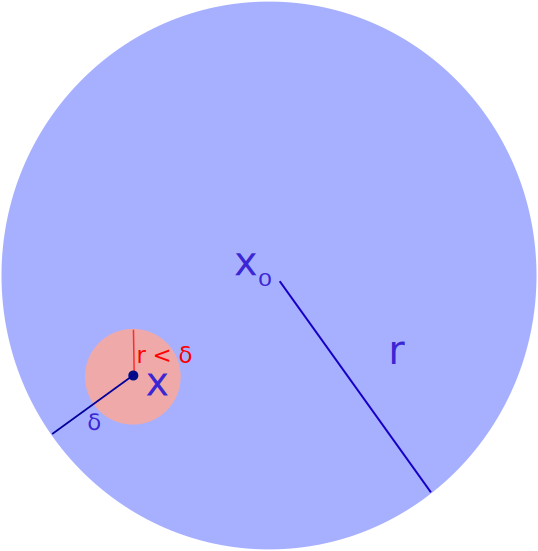
\includegraphics[width=350pt]{Schema2}
	\caption{Construction de la boule ouverte}
\end{figure}

\begin{myproposition}
	L'intersection de deux ouverts est un ouvert et toute réunion d'ouverts est un ouvert.
\end{myproposition}

\begin{myproof}
	Soient $U$ et $U'$ deux ouverts, montrons que $U \cap U'$ est un ouvert.
	
	Soit $x \in U \cap U'$, il existe $r>0$ et $r'>0$ tels que $\mathcal(B)(x, r) \subseteq U$ et $\mathcal{B}(x, r') \subseteq U'$.

	On pose $\widetilde{r}=\min(r, r')$ et on a $\mathcal{B}(x, \widetilde{r}) \subseteq U \cap U'$
	
	\cqfd
\end{myproof}

\begin{myproof}
	Soit $(U_i)_{i \in I}$ une famille d'ouverts, montrons que $U = \displaystyle \bigcup_{i \in I} U_i$ est un ouvert.
	
	Soit $x \in U$, alors il existe $i_0 \in I$ tel que $x \in U_{i_0}$, il existe donc $r$ tel que $\mathcal{B}(x, r) \subseteq U_{i_0}$ car $U_{i_0}$ est ouvert, d'où $\mathcal{B}(x, r) \subseteq U$.
	
	\cqfd
\end{myproof}

\begin{myproposition}
	Soit $X \subseteq E$, tout ouvert $U$ de $X$ s'écrit sous la forme $U=X \cap \widetilde{U}$, où $\widetilde{U}$ est un ouvert.
	
	De même pour tout fermé $F$ de $X$ s'écrit $F=X \cap \widetilde{F}$ où $\widetilde{F}$ est un fermé.
\end{myproposition}

\begin{myproof}
	Soit $\widetilde{U}$ un ouvert de $E$, alors $\widetilde{U} \cap X$ est un ouvert de $X$ par construction.
	
	Inversement soit $U$ ouvert de $X$, alors $\forall x \in U, ~ \exists r(x) > 0$ tel que $\mathcal{B}(x, r(x)) \cap X \subseteq U$
	
	Soit alors $\displaystyle \widetilde{U} = \bigcup_{x \in U} \mathcal{B}(x, r(x))$, alors $\widetilde{U}$ est un ouvert et $U = X \cap U$ 
\end{myproof}

\begin{mydef}
	Une suite à valeurs dans $E$ est dite \textit{convergente vers $x \in E$} si pour tout $\epsilon > 0$ il existe un rang $N$ tel que pour tout $n \geqslant N$ on ait $\|x_n-x\| < \epsilon$.
	
	On note $\lim\limits_{n} x_n = x$
\end{mydef}

\end{document}